\documentclass[../main.tex]{subfiles}
\graphicspath{{\subfix{../figures/}}}
%
\begin{document}
\section{观察者模式(Observer)}
观察者模式是对象行为模式,又称为发布-订阅模式、模型-视图(model-view)模式、源-监听器模式或者从属者模式。
观察者模式定义了一种一对多的依赖关系,让多个观察者对象同时监听某一个主题对象。这个主题对象在状态上发生变化时,会通知所有观察者对象,使它们能够自动更新自己。

根据观察者对象引用的存储地点,观察者模式的类图有微妙的区别。观察者模式类图(一)如下图所示:
%
\begin{figure}[H]
  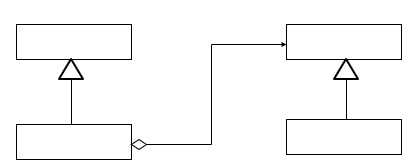
\includegraphics[width=0.30\textwidth]{29_1.jpg}
\end{figure}
%
观察者模式的简略类图(二)如下图所示
%
\begin{figure}[H]
  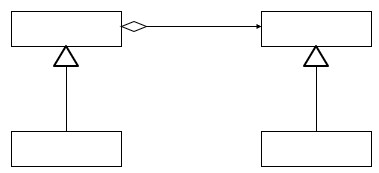
\includegraphics[width=0.30\textwidth]{29_2.jpg}
\end{figure}
%
Java语言提供的观察者模式的实现属于此种结构.
%
\subsection{观察者模式的结构}
以一个简单的示意性实现为例,讨论观察者模式的结构。如下图:
%
\begin{figure}[H]
  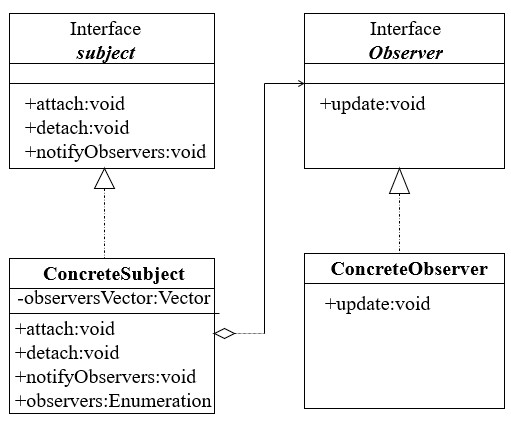
\includegraphics[width=0.50\textwidth]{29_3.jpg}
\end{figure}
%
可以看出,在这个观察者模式的实现里有下面这些角色:
\begin{itemize}
  \item 抽象主题(Subject)角色:主题角色把所有对观察者对象的引用保存在一个聚集里,每个主题都可以有任何数量的观察者。抽象主题提供一个接口,可以增加和删除观察者对象,主题角色又叫做抽象被观察者(Observable)角色。
  \item 具体主题(Concrete Subject)角色:负责管理具体主题的相关状态;在具体主题的状态改变时,给所有的观察者发出通知。具体主题又叫做具体被观察者(Concrete Observable)。具体主题角色负责实现对观察者引用的聚集的管理方法。
  \item 抽象观察者(Observer)角色:为所有的具体观察者定义一个接口,在得到主题的通知时更新自己。这个接口叫做通知/更新接口。
  \item 具体观察者(Concrete Observer)角色:实现抽象观察者角色所要求的更新接口,以便使本身的状态与主题 的状态相协调。
\end{itemize}
%
\lstinputlisting[language=java]{./code/29/1/Subject.java}
\lstinputlisting[language=java]{./code/29/1/ConcreteSubject.java}
\lstinputlisting[language=java]{./code/29/1/Observer.java}
\lstinputlisting[language=java]{./code/29/1/ConcreteObserver.java}
%
\subsubsection{另一种方案}
\begin{itemize}
  \item 考察主题对象的功能时,发现它必需使用一个java聚集来维护一个所有的观察者对象的引用.前一个方案中,管理这个聚集的是具体主题,因此在类图中存在从抽象观察者角色到具体主题角色的聚合连线.
  \item 但是所有具体主题管理聚集的方法都相同,因此可以将它移到抽象主题中.
  \item 第二种实现方案和第一种实现方案的主要区别就是代表存储观察者对象的聚合连线是从抽象主题到抽象观察者.
\end{itemize}
%
\begin{figure}[H]
  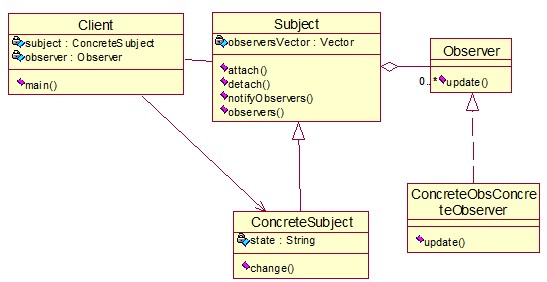
\includegraphics[width=0.50\textwidth]{29_4.jpg}
\end{figure}
%
\lstinputlisting[language=java]{./code/29/2/Subject.java}
\lstinputlisting[language=java]{./code/29/2/ConcreteSubject.java}
%
抽象观察者角色的源代码没有变化,不再列出.
%
\lstinputlisting[language=java]{./code/29/2/Client.java}
%
在运行时,客户端首先创建了具体主题的实例,以及一个观察者对象.然后,它调用主题对象的attach()方法,将这个观察者对象向主题对象登记,也就是将它加入到主题对象的聚集中去.
这时,客户端调用主题的业务逻辑方法,改变了主题对象的内部状态.主题对象在状态发生变化时,调用超类的notifyObservers()方法,通知所有登记过的观察者对象.其时序图如下:
%
\begin{figure}[H]
  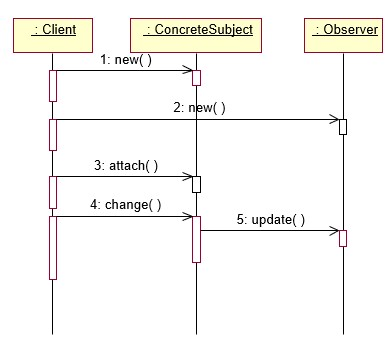
\includegraphics[width=0.50\textwidth]{29_5.jpg}
\end{figure}
%
\subsection{Java提供的对观察者模式的支持}
在java语言的java.util库里面,提供了一个Observable类以及一个Observer接口,构成Java语言对观察者模式的支持。
\begin{itemize}
  \item Observer接口: 这个接口只定义了一个方法,即update(Observable o, Object arg)方法。当被观察者对象的状态发生变化时,被观察者对象的notifyObserver()方法就会调用这一方法。
  \item Observable类: 被观察者类都是java.util.Observable类的子类。 java.util.Observable提供公开的方法支持观察者对象,这些方法中有两个对Observable子类非常重要:
    \begin{enumerate}
      \item setChanged():setChanged()被调用后会设置一个内部标记变量,代表被观察者对象的状态发生了变化.
      \item notifyObservers():这个方法被调用时,会调用所有登记过的观察者对象的update()方法,使这些观察者可以更新自己.
      \item addObserver():将观察者对象加入到聚集中.当有变化时,这个聚集可以告诉notifyObservers()方法哪些观察者对象需要通知.
    \end{enumerate}
\end{itemize}
%
\lstinputlisting[language=java]{./code/29/3/Observable.java}
%
Observable也被称为主题对象.一个被观察者对象有数个观察者对象,每个观察者对象实现Observer接口.被观察者对象发生变化时,会调用Observable的notifyObservers方法,此方法调用所有的具体观察者的update()方法,从而使所有的观察者都被通知更新自己.使用java语言提供的观察者模式的支持类图如下:
%
\begin{figure}[H]
  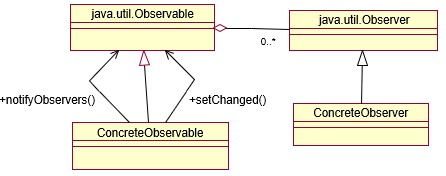
\includegraphics[width=0.50\textwidth]{29_6.jpg}
\end{figure}
%
\subsection{怎样使用Java对观察者模式的支持}
本节给出一个非常简单的例子。在这个例子中,被观察者对象叫做Watched;而观察者对象叫做Watcher。Watched对象继承自java.util.Observable类;而Watcher对象实现了java.util.Observer接口。另外有一个对象Tester,扮演客户端的角色.这个系统简单的结构图如下:
%
\begin{figure}[H]
  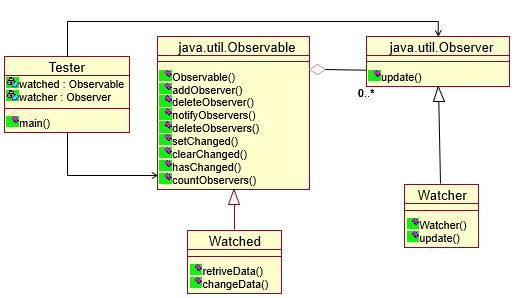
\includegraphics[width=0.50\textwidth]{29_7.jpg}
\end{figure}
%
\lstinputlisting[language=java]{./code/29/4/Watched.java}
\lstinputlisting[language=java]{./code/29/4/Watcher.java}
\lstinputlisting[language=java]{./code/29/4/Tester.java}
%
可以看出,虽然客户方将Watched对象的内部状态赋值了四次,但是值的改变只有三次,代码清单如下:
%
\begin{itemize}
  \item watched.changeData("In C, we create bugs.");
  \item watched.changeData("In Java, we inherit bugs.");
  \item watched.changeData("In Java, we inherit bugs.");
  \item watched.changeData("In Visual Basic, we visualize bugs.");
\end{itemize}
%
相应地,Watcher对象响应了三次改变。运行结果如下:
%
\begin{itemize}
  \item Data has been changed to: ‘In C, we create bugs.’
  \item Data has been changed to: ‘In Java, we inherit bugs.’
  \item Data has been changed to: ‘In Visual Basic, we visualize bugs.’
\end{itemize}
%
系统的活动时序图如下:
%
\begin{figure}[H]
  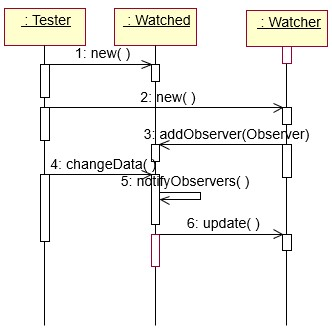
\includegraphics[width=0.40\textwidth]{29_8.jpg}
\end{figure}
%
Tester对象首先创建了Watched和Watcher对象。在创建Watcher对象时,将Watched对象作为参量传入;然后Tester对象调用Watched对象的changeData()方法,触发Watched对象的内部状态变化;Watched对象进而通知实现登记过的Watcher对象,也就是调用的update()方法。
%
\subsection{Java中的DEM事件机制}
\textbf{AWT中的DEM机制}:
在AWT1.1版本以及以后的各个版本中,事件处理模型均为基于观察者模式的委派事件模型(Delegation Event Model或DEM)。
在DEM中,主题角色负责发布事件,观察者角色向特定的主题订阅它所感兴趣的事件。当一个具体主题产生一个事件时,它就会通知所有感兴趣的订阅者。
在DEM模型中发布者叫做事件源,而订阅者叫做事件监听器。
%
\begin{lstlisting}[language=java]
new java.awt.Button(new ActionListner(){
  void actionPerform(){
    // ...
  }
});
\end{lstlisting}
%
\subsection{观察者模式的优缺点}
\begin{itemize}
  \item 优点:观察者模式在被观察者和观察者之间建立一个抽象的耦合。观察者模式支持广播通信。
  \item 缺点:如果一个被观察者有很多的观察者,将所有的观察者都通知到会花费很多时间。如果在被观察者之间有循环依赖,被观察者会触发它们之间进行循环调用,导致系统崩溃。
    虽然观察者随时知道所观察的对象发生了变化,但是观察者模式没有相应的机制使观察者知道所观察的对象是怎样发生变化的。
\end{itemize}
%
\end{document}
